\documentclass[onecolumn]{article}
%\usepackage{url}
%\usepackage{algorithmic}
\usepackage[a4paper]{geometry}
\usepackage{datetime}
\usepackage{hyperref}
\usepackage[margin=2em, font=small,labelfont=it]{caption}
\usepackage{graphicx}
\usepackage{mathpazo} % use palatino
\usepackage[scaled]{helvet} % helvetica
\usepackage{microtype}
\usepackage{amsmath}
\usepackage{subfigure}
\usepackage{listings}
\usepackage{float}
\usepackage{xcolor} %red, green, blue, yellow, cyan, magenta, black, white
\usepackage{graphicx}
\usepackage[font=small,labelfont=bf]{caption}
\renewcommand{\thefigure}{\arabic{section}.\arabic{figure}}
\graphicspath{ {pictures/} }
\definecolor{mygreen}{RGB}{28,172,0} % color values Red, Green, Blue
\definecolor{lightgray}{gray}{0.9}
\definecolor{mylilas}{RGB}{170,55,241}
\newcommand{\inlinecode}[2]{\colorbox{lightgray}{\lstinline[language=#1]$#2$}}


% Letterspacing macros
\newcommand{\spacecaps}[1]{\textls[200]{\MakeUppercase{#1}}}
\newcommand{\spacesc}[1]{\textls[50]{\textsc{\MakeLowercase{#1}}}}
\newcommand{\inline}[1]{\colorbox{lightgray}{\lstinline[basicstyle=\ttfamily\color{brown}]|#1|}}

\title{\spacecaps{Lab report: Lab 7 }\\
Application of box models to Upper Danube catchment simulation\\\normalsize \spacesc{Modeling of Physical Systems} }

\author{Patryk Gałczyński}
%\date{\today\\\currenttime}
\date{\today}


\begin{document}
\lstset{language=Matlab,%
    %basicstyle=\color{red},
    %breaklines=true,%
    morekeywords={matlab2tikz},
    keywordstyle=\color{blue},%
    morekeywords=[2]{1}, keywordstyle=[2]{\color{black}},
    identifierstyle=\color{black},%
    stringstyle=\color{mylilas},
    commentstyle=\color{mygreen},%
    showstringspaces=false,%without this there will be a symbol in the places where there is a space
    numbers=left,%
    numberstyle={\small \color{black}},% size of the numbers
    numbersep=9pt, % this defines how far the numbers are from the text
    emph=[1]{for,end,break},emphstyle=[1]\color{red}, %some words to emphasise
    %emph=[2]{word1,word2}, emphstyle=[2]{style},    
}

\maketitle


\section{Aim of laboratory}
\large
Main goal of this laboratory was to estimate mean residence time of water in Danube river with black-box model using exponential transit function.

\section{Simulation description}
As laboratory aim states, it is required to estimate mean residence time of water in Danube river. To achieve that, black box model is being used - which means, system won't be  controlled directly, but only by adjusting its input parameters according to obtained output, without knowledge about its internals.

To model such phenomena, calculation of concentration of the tracer - Tritium 3H in this particular case - can be utilized. In this case, mathematical formula describing that model looks as follows:

\begin{equation}
	C(t) = \int_{- \infty}^{t} C_{in}(t') \cdot g(t - t') \cdot e^{-\lambda \cdot (t - t')} dt'
\end{equation}
Where:
\begin{itemize}
    \item t - time variable
	\item $C(t)$ - output function
    \item $C_{in}(t')$ - input function
    \item $g(t - t') = \frac{e^{\frac{-(t-t')}{t_t}}}{t_t}$ - exponential time transit distribution function
    \item $t_t$ - mean residence time
    \item $\lambda = 4.696 * 10^{-3}$ - radioactive decay constant
\end{itemize}

To evaluate such model, two data sets were provided:
\begin{enumerate}
	\item \inlinecode{matlab}{opady.prn} - file that contains input function values
    \item \inlinecode{matlab}{dunaj.prn} - file with calculated amount of tracer in Danube river in Vienna station (output to compare output to)
\end{enumerate}

\newpage
\section{Implementation and results}

\subsection{Input and output data analysis}
Plotting provided datasets, gives the following chart:\\
\noindent\makebox[\textwidth]{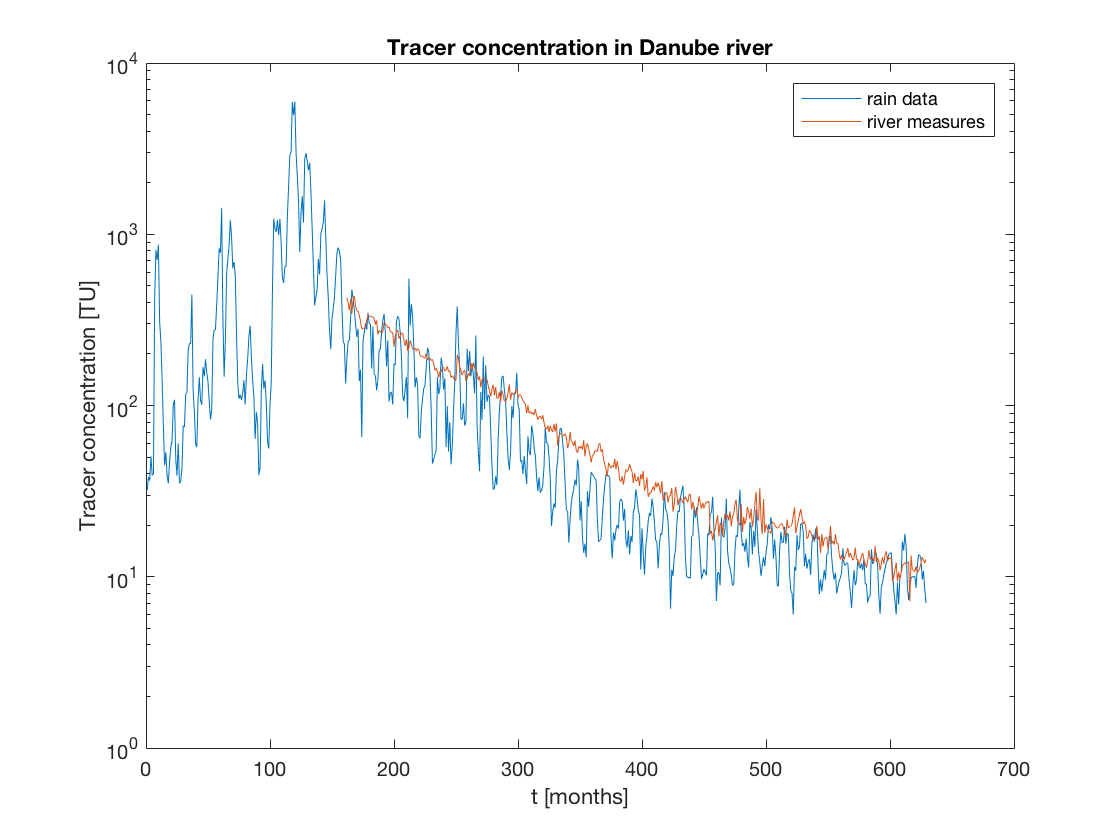
\includegraphics[scale=0.5]{1.png}}
It is worth noticing that first 160 river measures are missing, however, they could be extrapolated from rain data. Other fact worth mentioning is that, it is clearly visible (not so obvious at the first glance), that river data is similar and slightly shifted to the right comparing with rain measures. This shift between input and output data can be used for mean residence time calculation.  

\subsection{Convolution integral}
To calculate previously mentioned convolution integral with exponential time transit distribution function, the following matlab function were developed:
\begin{lstlisting}[language=Matlab,frame=single,label={lst:autocorr},breaklines=true,caption={Convolutional integral implementation with exponential transit function}]
function sumsum = easy_integral(c_in, i, dt, tt, lambda)
    sum = 0;
    t = i * dt;
    for j = 1:i-1
        tp = j*dt;
        sum = sum + c_in(j) * ...
                    tt^(-1) * ...
                    exp(-1 * (t - tp) / tt) * ... 
                    exp(-1 * lambda * (t - tp));
    end;
    sumsum = sum * dt;
end
\end{lstlisting}
It takes as parameters:
\begin{enumerate}
	\item \inlinecode{matlab}{c_in} -  input function values vector;
    \item \inlinecode{matlab}{i} - timestamp for which to calculate;
    \item \inlinecode{matlab}{dt} - timestep;
    \item \inlinecode{matlab}{tt} - mean residence time;
    \item \inlinecode{matlab}{lambda} - radioactive decay constant.
\end{enumerate}
And returns calculated sum. Therefore, this function was run multiple times in the \inlinecode{matlab}{for loop} with the following parameters:
\begin{lstlisting}[language=Matlab,frame=single,label={lst:autocorr},breaklines=true,caption={Convolutional integral implementation with exponential transit function}]
    rain = importdata('opady.prn');
    dunaj_river = importdata('dunaj.prn');
    num = rain(end, 1);
    tt = 10;                    % month
    lambda = 4.696e-3;          % 1/month?
    dt = rain(2,1) - rain(1,1); % month
    output = zeros(num,1);      % vector with output values



    for i= 1:num
        output(i) = easy_integral(rain(:,2), i, dt, tt, lambda);
    end
    
    figure;
    semilogy(dunaj_river(:,2));
    hold on;
    semilogy(output1);
\end{lstlisting}
With presented result: \\
\noindent\makebox[\textwidth]{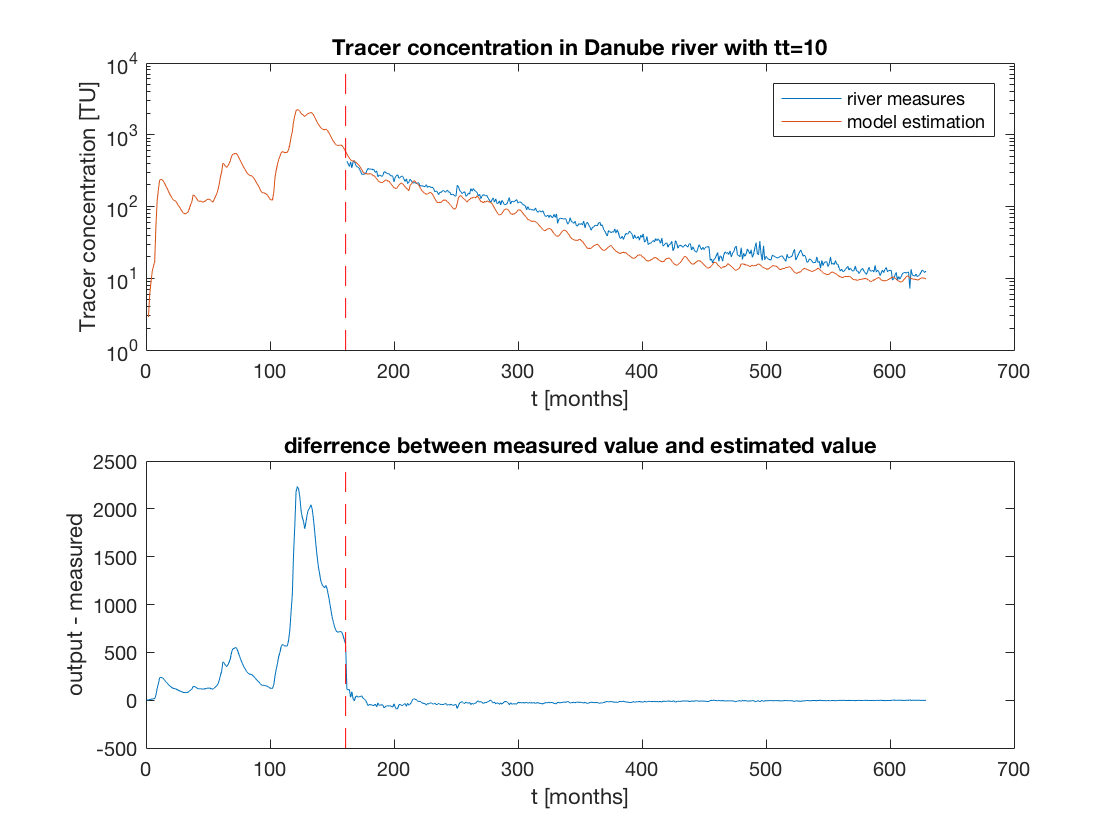
\includegraphics[scale=0.5]{2.png}}

One can conclude, that model approximates real values quite well, looking at difference between model output values and real datapoints. However, it still can be done better - tt value in this case, was guessed. 

\subsection{Calculating possible tt values}
One way, to obtain tt value which suits well this model, is to check the next values occurring in the sequence while error value decrees. Example script performing such action is available below:
\begin{lstlisting}[language=Matlab,frame=single,label={lst:autocorr},breaklines=true,caption={Convolutional integral implementation with exponential transit function}]

rain = importdata('opady.prn');
dunaj_river = importdata('dunaj.prn');
lambda = 4.696e-3;          % 1/month?
dt = rain(2,1) - rain(1,1); % month
mean_residence = [];
old_rmse = 0;

for tt = 1:1000
    num = rain(end, 1);

    output = zeros(num,1);      % vector with output values
    for i= 1:num
        output(i) = easy_integral(rain(:,2), i, dt, tt, lambda);
    end
    
    % count error, excluding values that does not make sense
    errors = (dunaj_river(161:num,2) - output(161:num));
    errors = errors.^2;
    
    % root mean square error
    rmse = sqrt(sum(errors)/num);
    if tt == 1
        old_rmse = rmse;
    else
        if rmse > old_rmse
            disp(tt);
            break;
        else
            old_rmse = rmse;
        end
    end
end

\end{lstlisting}

This method resulted in conclusion that tt = 8 is most suitable. Which sounds reasonable.

More sophisticated method to check for good tt value is to minimize rooted square error of output and measured values. Achieving that is simple as:
\begin{lstlisting}[language=Matlab,frame=single,label={lst:autocorr},breaklines=true,caption={Convolutional integral implementation with exponential transit function}]

rain = importdata('opady.prn');
dunaj_river = importdata('dunaj.prn');
lambda = 4.696e-3;          % 1/month?
dt = rain(2,1) - rain(1,1); % month
mean_residence = [];

for tt = 1:1000
    num = rain(end, 1);

    output = zeros(num,1);      % vector with output values
    for i= 1:num
        output(i) = easy_integral(rain(:,2), i, dt, tt, lambda);
    end
    
    % count error, excluding values that does not make sense
    errors = (dunaj_river(161:num,2) - output(161:num));
    errors = errors.^2;
    
    % root mean square error
    rmse = sqrt(sum(errors)/num);
    mean_residence(tt,1) = tt;
    mean_residence(tt,2) = rmse;
end

% find tt with minimal RMSE
[val, idx] = min(mean_residence);
disp(val);
disp(idx);
\end{lstlisting}

\newpage
resulting in:
\begin{lstlisting}[language=Matlab,frame=single,label={lst:autocorr},breaklines=true,caption={Convolutional integral implementation with exponential transit function}]
>> river_flow
          1.00         31.04

          1.00        217.00
\end{lstlisting}
Which looks ridiculous, nonetheless, this is tt which gives the smallest RMSE. But, if one would take a look into chart presenting function of RMSE depending on tt value, then it is clearly visible that in fact 217 is global minimum of this function, however local minimum in 
$tt = 8$ is more likely to be true. \\
\noindent\makebox[\textwidth]{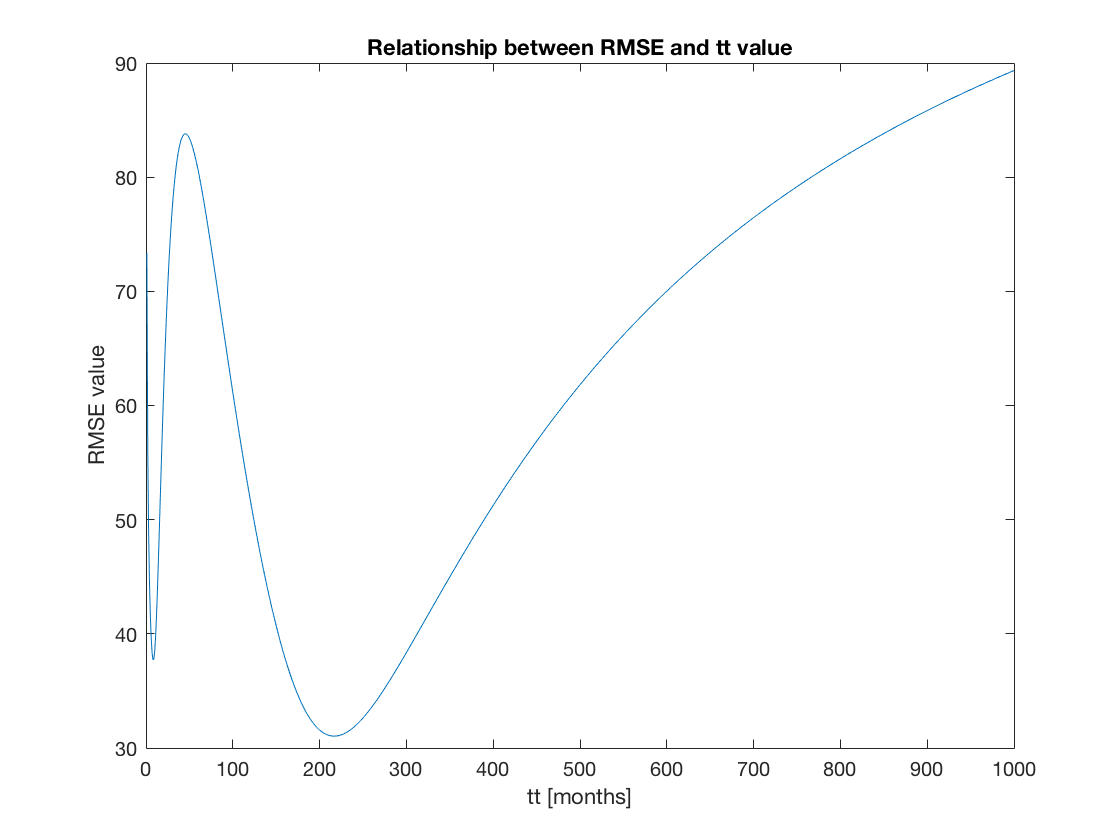
\includegraphics[scale=0.5]{3.png}}

\newpage
\begin{lstlisting}[language=Matlab,frame=single,label={lst:autocorr},breaklines=true,caption={Convolutional integral implementation with exponential transit function}]
% check for local minimum at the beginning
>> min(mean_residence(1:100,:))
          1.00         37.73

          1.00          8.00
\end{lstlisting}

To check, whether these tt values makes sense, another chart with measured values compared to model values with tt = 217 and tt = 8 were developed:
\noindent\makebox[\textwidth]{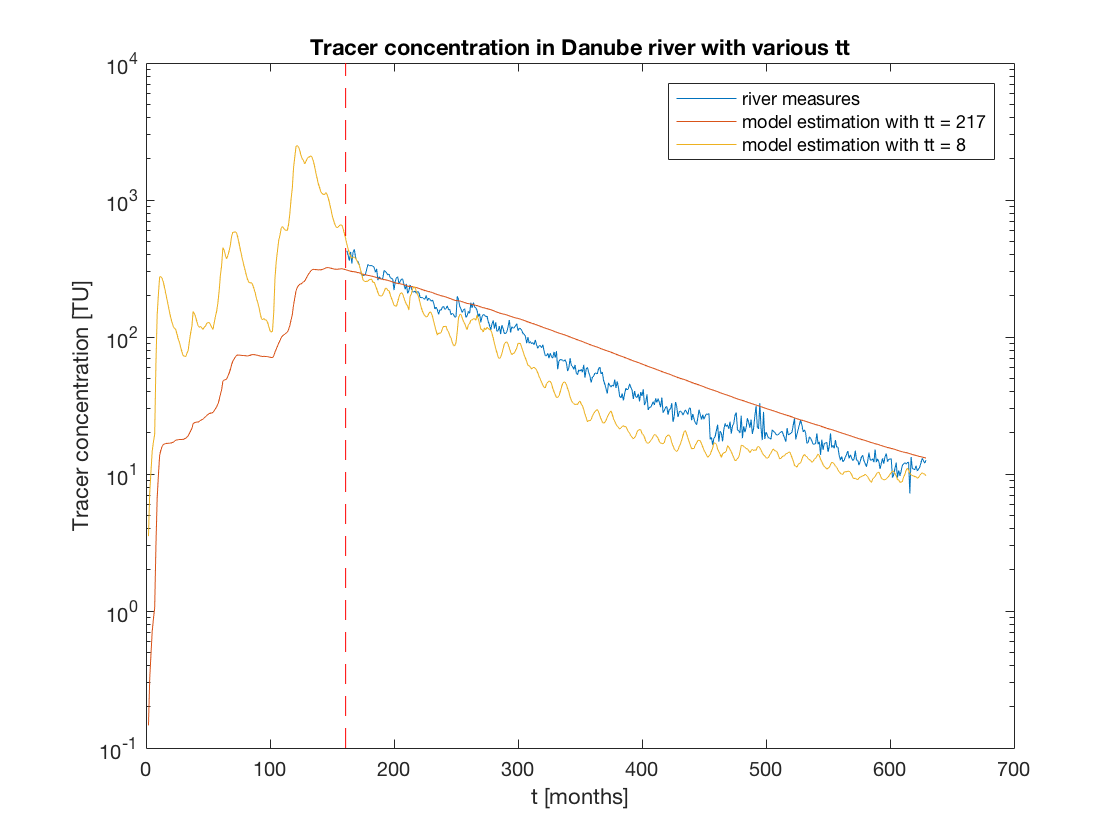
\includegraphics[scale=0.5]{4.png}}

\subsection{Results comparison}
Both methods resulted in similar results stating that mean residence time is equal to 8 months. However, trial error method seems to be more primitive and vulnerable for local minima, which in this case turned out to be helpful, but inverse modeling (minimizing rmse in this case) looked more promising, and actually proved first result, but not directly, because it found global minimum which does not make much sense in this case (or is it?)

\section{Conclusion}
This report covered simplified methods to calculate the mean residence time of water in the upper part of the Danube river using black box modeling technique with exponential transit function. Results obtained by two different methods agree with each other, and looks reasonable from author perspective. Output values produced by generated model fits not-so-well-but-acceptable provided example.
\end{document}